
%(BEGIN_QUESTION)
% Copyright 2011, Tony R. Kuphaldt, released under the Creative Commons Attribution License (v 1.0)
% This means you may do almost anything with this work of mine, so long as you give me proper credit

This schematic diagram shows a set of level switches used to detect dangerously low and high liquid level conditions in a process vessel.  The 3.8 foot switch maintains power to the ``system enable'' solenoid only if there is at least that much liquid in the vessel, shutting down the system if the liquid level ever drops below that value.  The 5.5 foot switch triggers a high-level alarm lamp if the liquid level exceeds that value.

$$\includegraphics[width=15.5cm]{i03448x01.eps}$$

Unfortunately, the circuit as designed provides no means to {\it bypass} or {\it disable} these protective functions if ever a liquid level switch needs to be removed from the circuit for repair, calibration, or replacement while the system is running.  As it stands right now, any technician trying to handle either of these switches while the process is running risks either shutting it down or tripping the high-level alarm.

Modify this schematic diagram to include two toggle switches, one to disable the low-level shutdown and the other to disable the high-level alarm.  The switch symbols available for you to use are displayed above the diagram for your reference.  Simply sketch the appropriate toggle switch type in the appropriate location within the schematic diagram to implement the needed bypass functions.  The toggle switches should be drawn in such a way that their ``normal'' states allow the level switches to perform their protective functions.

\underbar{file i03448}
%(END_QUESTION)





%(BEGIN_ANSWER)

5 points for each correctly-drawn bypass switch:

$$\includegraphics[width=15.5cm]{i03448x02.eps}$$

%(END_ANSWER)





%(BEGIN_NOTES)

{\bf This question is intended for exams only and not worksheets!}.

%(END_NOTES)


